%%%%%%%%%%%%%%%%%%%%%%%%%%%%%%
%Section
%%%%%%%%%%%%%%%%%%%%%%%%%%%%%%
\subsection{Command and Control}
\label{ssec:background_c2}

Command and Control (C2) is the exercise of authority and direction by a properly designated commander over assigned and attached forces in the accomplishment of a mission~\citep{dod01}. \citet{Alberts2006} \color{black}extend \color{black} this definition including the efforts of a set of entities, i.e., members or organizations, and resources, including information, in order to achieve a goal or result. Such a definition includes information as one of its component elements that travel on a network structure \color{black}to satisfy \color{black} the context requirements and mission details. According to~\citet{Stanton2007} and~\citet{Mason2001}, C2 relies on information and awareness sharing rather than simply data broadcast. 

Created in the military domain, the C2 concepts were extended to become applicable  to multiple domains through the process that increases the action power through a shared awareness. This awareness can be synchronized using a specific network structure and organization \color{black} to create entity interactions, \color{black} so called Network Centric Warfare (NCW) - USA -  or Network Enabled Capabilities (NEC) - England~\citep{Alberts2000}. \color{black} Based on the NEC paradigm,~\citet{FRANCE2014,nato01} present five approaches to C2 described as follows:
\begin{itemize}
    \item \textit{Conflicted}: there is no allocation of decision rights, no interaction among entities, and the entities have only internal information; 

    \item \textit{De-Conflicted}: there are constraints to the allocation of decision rights, the interactions among entities are very limited with limited information exchanges restricted to constraints and joints;

    \item \textit{Coordinated}: the allocation of decision rights follows a coordination plan, the patterns of interaction are limited and focused, and there is additional information;

    \item \textit{Collaborative}: the allocation of decision rights follows a collaborative process and shared plan, the entities’ interaction is broad, and there is additional information across collaborative areas;

    \item \textit{Edge}: there is a self allocation of decision rights dynamically, the entity interactions are unlimited, and all information is available.
\end{itemize}
\color{black}

From a structure where there is no information and decision sharing (Conflicted) to a fully connected structure where all entities share information and decision capability (Edge), these approaches combine different levels of decision making, data sharing, and information. Each one looks for different entities' awareness levels obtained through a suitable communications improvement to deal with more complex scenarios and mission conditions~\citep{nato01,Power01}. \color{black}This complexity increases with context changes, that is, changes in the environment, in the mission, or in the entities. Particularly, the environment involves everything that surrounds the entities, such as  enemies' characteristics, weather, and environmental conditions\color{black}. Based on this, C2 Agility emerges as the system's ability to deal with such context changes, \color{black}adapting to new requirements in order to continue execution of the tasks\color{black}~\citep{FRANCE2014}. According to~\citet{Alberts2006}, this C2 Agility is the combination of the following elements:

\begin{center}
\fbox{\begin{minipage}{30em}
\begin{itemize}

    \item \textbf{C2 Approach Agility}: members' and structure adaptation within the operated C2 Approach to deal with context changes;
    
    \item \textbf{C2 Maneuver Agility}: C2 Approach change to obtain a different awareness level to deal with context changes.

\end{itemize}
\end{minipage}}    
\end{center}

Each C2 Approach provides a different communication structure with a distinct awareness level \X{suitable} for specific contexts.~\citet{nato01} highlights that there is no best unique solution to satisfy all requirements of a given circumstance.



%%%%%%%%%%%%%%%%%%%%%%%%%%%%%%
%Section
%%%%%%%%%%%%%%%%%%%%%%%%%%%%%%
\subsection{Channel System}
\label{ssec:background_cs}


\citet{MC01} define channel systems (CS) as parallel systems with processes running independently that communicate via channels, which are first-in, first-out buffers that may contain messages. CS are assumed to be closed, that is, inter-processes communication is only allowed in the system, but not outside it. Each parallel process is defined by a program graph (PG), which is a representation of the system's behavior, abstracting over its transition system semantics. Equation~\ref{eq:cs01} defines the CS formed by a sequence of $n$ PGs running in parallel within the same system:


\begin{equation}
    \label{eq:cs01}
    CS=[PG_1|PG_2|...|PG_n]
\end{equation}

Figure~\ref{fig:pg_example} illustrates a program graph that models a print server that reads an image file from a buffer and sends it to a printer. It is defined by the tuple\\ $\mathit{PG=(Loc,Act,Effect,\hookrightarrow,Loc_0,g_0)}$, where



\begin{itemize}
    \item $Loc=\{wait, print, load, cancel\}$ is the set of locations, that is,     nodes that have a control function;
    \item $Act=\{start, flush\}$ is the set of actions;
    \item $\mathit{Effect}$ is the function modeling the effect of actions on the state of the PG, i.e., it's what the actions do;
    \item $\hookrightarrow$ is the conditional transition from a location $l$ to a location $l'$, represented by $l\xhookrightarrow[]{g:\alpha}l'$, where an action $\alpha \in Act$ is performed when a condition, so-called guard, $g$ is satisfied;
    \item $Loc_0=\{wait\}$ is the set of initial locations;
    \item $g_0$ is the initial condition on the variables of the system, \X{required for starting the CS.}
\end{itemize}

\begin{figure}[!ht]
    \centering
    \color{black}
    \scalebox{.8}{

\tikzset{every picture/.style={line width=0.75pt}} %set default line width to 0.75pt        

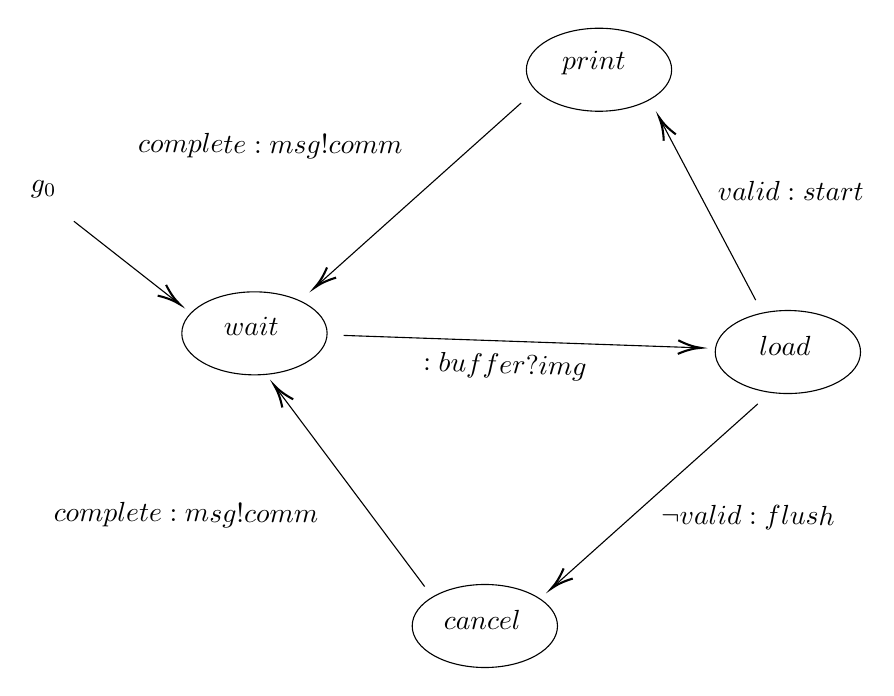
\begin{tikzpicture}[x=0.75pt,y=0.75pt,yscale=-1,xscale=1]
%uncomment if require: \path (0,331); %set diagram left start at 0, and has height of 331

%Shape: Ellipse [id:dp8321971521800935] 
\draw   (198,301) .. controls (198,289.95) and (213.67,281) .. (233,281) .. controls (252.33,281) and (268,289.95) .. (268,301) .. controls (268,312.05) and (252.33,321) .. (233,321) .. controls (213.67,321) and (198,312.05) .. (198,301) -- cycle ;
%Shape: Ellipse [id:dp9498214710995798] 
\draw   (87,160) .. controls (87,148.95) and (102.67,140) .. (122,140) .. controls (141.33,140) and (157,148.95) .. (157,160) .. controls (157,171.05) and (141.33,180) .. (122,180) .. controls (102.67,180) and (87,171.05) .. (87,160) -- cycle ;
%Shape: Ellipse [id:dp5125970438473768] 
\draw   (344,169) .. controls (344,157.95) and (359.67,149) .. (379,149) .. controls (398.33,149) and (414,157.95) .. (414,169) .. controls (414,180.05) and (398.33,189) .. (379,189) .. controls (359.67,189) and (344,180.05) .. (344,169) -- cycle ;
%Shape: Ellipse [id:dp8080305675784576] 
\draw   (253,33) .. controls (253,21.95) and (268.67,13) .. (288,13) .. controls (307.33,13) and (323,21.95) .. (323,33) .. controls (323,44.05) and (307.33,53) .. (288,53) .. controls (268.67,53) and (253,44.05) .. (253,33) -- cycle ;
%Straight Lines [id:da6100445878394302] 
\draw    (35,106) -- (84.43,144.77) ;
\draw [shift={(86,146)}, rotate = 218.11] [color={rgb, 255:red, 0; green, 0; blue, 0 }  ][line width=0.75]    (10.93,-3.29) .. controls (6.95,-1.4) and (3.31,-0.3) .. (0,0) .. controls (3.31,0.3) and (6.95,1.4) .. (10.93,3.29)   ;
%Straight Lines [id:da35540329737679166] 
\draw    (132.7,186.6) -- (204,282) ;
\draw [shift={(131.5,185)}, rotate = 53.22] [color={rgb, 255:red, 0; green, 0; blue, 0 }  ][line width=0.75]    (10.93,-3.29) .. controls (6.95,-1.4) and (3.31,-0.3) .. (0,0) .. controls (3.31,0.3) and (6.95,1.4) .. (10.93,3.29)   ;
%Straight Lines [id:da29699699994491846] 
\draw    (165,161) -- (335,166.93) ;
\draw [shift={(337,167)}, rotate = 182] [color={rgb, 255:red, 0; green, 0; blue, 0 }  ][line width=0.75]    (10.93,-3.29) .. controls (6.95,-1.4) and (3.31,-0.3) .. (0,0) .. controls (3.31,0.3) and (6.95,1.4) .. (10.93,3.29)   ;
%Straight Lines [id:da31457893798010017] 
\draw    (317.93,57.77) -- (363.5,144) ;
\draw [shift={(317,56)}, rotate = 62.15] [color={rgb, 255:red, 0; green, 0; blue, 0 }  ][line width=0.75]    (10.93,-3.29) .. controls (6.95,-1.4) and (3.31,-0.3) .. (0,0) .. controls (3.31,0.3) and (6.95,1.4) .. (10.93,3.29)   ;
%Straight Lines [id:da8819741384484475] 
\draw    (250.5,49) -- (152.49,136.67) ;
\draw [shift={(151,138)}, rotate = 318.19] [color={rgb, 255:red, 0; green, 0; blue, 0 }  ][line width=0.75]    (10.93,-3.29) .. controls (6.95,-1.4) and (3.31,-0.3) .. (0,0) .. controls (3.31,0.3) and (6.95,1.4) .. (10.93,3.29)   ;
%Straight Lines [id:da0480873078365871] 
\draw    (364.5,194) -- (266.49,281.67) ;
\draw [shift={(265,283)}, rotate = 318.19] [color={rgb, 255:red, 0; green, 0; blue, 0 }  ][line width=0.75]    (10.93,-3.29) .. controls (6.95,-1.4) and (3.31,-0.3) .. (0,0) .. controls (3.31,0.3) and (6.95,1.4) .. (10.93,3.29)   ;

% Text Node
\draw (13,85) node [anchor=north west][inner sep=0.75pt]    {$g_{0}$};
% Text Node
\draw (106,151) node [anchor=north west][inner sep=0.75pt]    {$wait$};
% Text Node
\draw (364,160) node [anchor=north west][inner sep=0.75pt]    {$load$};
% Text Node
\draw (269,23) node [anchor=north west][inner sep=0.75pt]    {$print$};
% Text Node
\draw (212,292) node [anchor=north west][inner sep=0.75pt]    {$cancel$};
% Text Node
\draw (202.31,167.58) node [anchor=north west][inner sep=0.75pt]  [rotate=-1.82]  {$\text{:buffer} ?img$};
% Text Node
\draw (344.08,85.43) node [anchor=north west][inner sep=0.75pt]  [rotate=-0.23]  {$valid:start$};
% Text Node
\draw (316.74,241.51) node [anchor=north west][inner sep=0.75pt]  [rotate=-0.23]  {$\neg valid:flush$};
% Text Node
\draw (64.75,62.43) node [anchor=north west][inner sep=0.75pt]  [rotate=-0.23]  {$complete:msg!comm$};
% Text Node
\draw (24.08,240.1) node [anchor=north west][inner sep=0.75pt]  [rotate=-0.23]  {$complete:msg!comm$};


\end{tikzpicture}}
    \caption{Program Graph example with 4 locations modeling a print server.}
    \label{fig:pg_example}
\end{figure}

Specific actions model communication among program graphs. Action $ch!x$ writes message $x$ in channel $ch$, whereas action $ch?x$ reads the message from the channel and stores it in variable $x$. In either case, the variables and messages types must be compatible. For example, in Figure~\ref{fig:pg_example}, from locations $wait$ to $load$, data is read from a channel called \textit{buffer} and stored in variable \textit{img}. As there is no guard condition before the two points, and no alternative action from location \textit{wait}, the operation always occurs when there is data on the channel.  The write operation occurs in locations \textit{print} and \textit{cancel}, where the variable \textit{msg}'s content is written in channel \textit{comm} and is available to be read by another PG within the same CS. In such a case, these operations occur when the the guard condition  \textit{complete} is satisfied.

The channel capacity \X{for} storing messages, denoted by $cap(ch)$,  is defined by its buffer size. When $cap(ch) > 0$, communication occurs asynchronously. Otherwise, \emph{handshaking} takes place, that is,  read and write operations occur synchronously. In the previous example, we have that $\mathit{cap(buffer)=0}$  to make the PG stop and wait for information arrival at channel \textit{buffer}. 

Besides, in Figure~\ref{fig:pg_example},  by executing the transition from \textit{wait} to \textit{load}, the process reads an image from the channel called \textit{buffer} and \X{stores} it in the variable \textit{img}, going from location \textit{wait} to \textit{load}. Next, the server can print \textit{img} with the image file, if the condition \textit{valid} is satisfied, i.e., $valid=true$. In such a case, the \textit{start} action is performed, and the next location reached is \textit{print}. Otherwise, identifying some problem, it cancels the operation and goes to the \textit{cancel} location, running the \textit{flush} action.

%\begin{table}[ht!]
	\small
	\fontsize{11}{11}\selectfont
	\centering
	\caption{Channels Capacity - cap(c)}
	\label{table:channel}
	
%	\begin{tabularx}{.9\textwidth}{X{0.4\linewidth}X{0.5\linewidth}}
    \begin{tabularx}{.8\textwidth}{cX}
	\hline
		
		\textbf{Capacity}
		& \textbf{Description} \\ [1ex]
	\hline	
	
	\\$cap(c)>0$ & There is a delay  between the messages transmission and receipt (Asynchronous channel)
	\\[1ex] \\
	
	\\ $cap(c)=0$ & The message transmission and receipt corresponds to a handshaking (Synchronous channel) 
	\\[1ex] \\
	\hline
	\end{tabularx}
\end{table} 

